\def\logipchisq{\ensuremath{\log_{10}\chi^2_{\text{IP}}~}}
\section{Data sets and selections}
\label{sec:data}
\subsection{Data sets}
The data for this analysis was \plead data collected by \lhcb detector at late 2016,
including two different configurations due to the asymmetry of collisions:
forward (Fwd) collision(\proton beam coming from upstream of \velo)
and backward (Bwd) collision(Pb beam coming from upstream of \velo).
The configurations, corresponding to positive and negative rapidity regions respectively,
are illustrated in the two pannels of Fig.~\ref{fig:FwdBwd}:
\begin{figure}[htbp]
    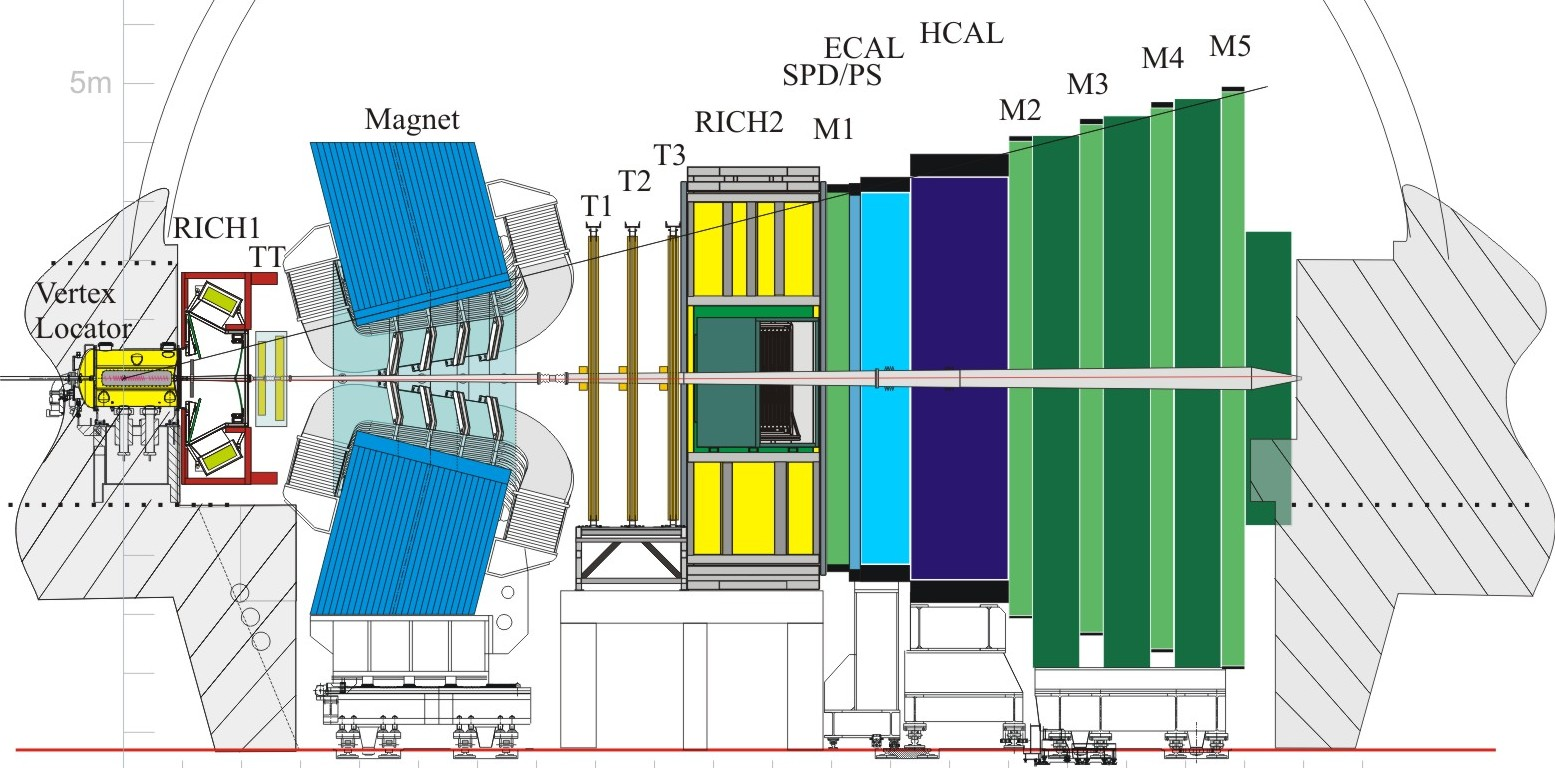
\includegraphics[width=0.48\linewidth]{plead1}
    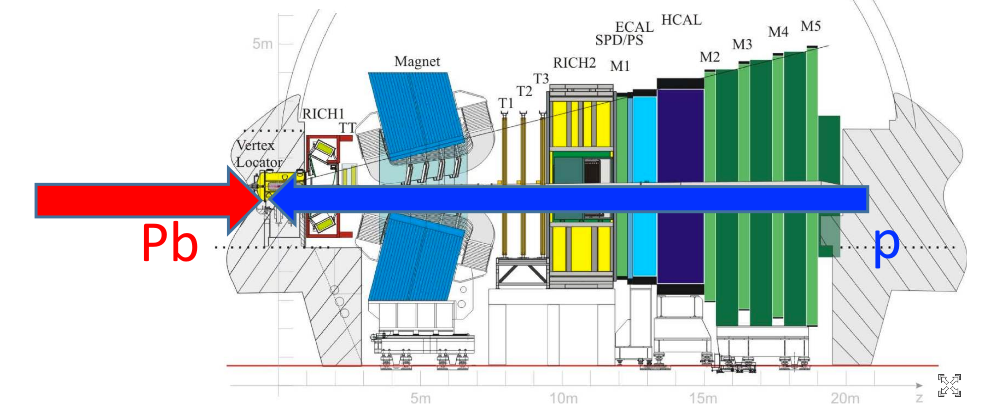
\includegraphics[width=0.48\linewidth]{plead2}
    \caption{Skeches of the two beam configurations of $p$Pb data taking,
    left for Fwd($p$Pb) and right for Bwd(Pb$p$).}
    \label{fig:FwdBwd}
\end{figure}
The integrated luminosity for Fwd collision is 12.18 $\pm$ 0.32 \invnb and 18.57 $\pm$ 0.46\invnb for Bwd.
The centre-of-mass energy per nucleon pair \sqsnn corresponds to 8.16\tev.
The bookkeeping paths for Fwd and Bwd are:
\begin{align*}\tiny
    &\text{/LHCb/Protonion16/Beam6500GeV-VeloClosed-MagDown/Real Data}\\
    &\text{/Turbo03pLead/94000000/TURBO.MDST}; \\
    &\text{/LHCb/Ionproton16/Beam6500GeV-VeloClosed-MagDown/Real Data}\\
    &\text{/Turbo03pLead/94000000/TURBO.MDST}.
\end{align*}

The data samples are triggered online in three levels.
The first level (Level-0) is a hardware level trigger {\tt L0SPD} for $p$Pb data,
which requires at least ones hit in the SPD detector.
Thus it is an minmum biased trigger with $\varepsilon_\mathrm{L0} \approx 1$.
The (software) high-level triggers HLT1 and HLT2 provide real time reconstruction and selection
of tracks and particles.
For hadron-final-state channels, such as $\decay{\Dz}{\Km\pip}$ and $\decay{\Lc}{\proton\Km\pip}$,
the HLT1 triggers are {\tt{Hlt1TrackMVADecision\_TOS}} or {\tt{Hlt1TwoTrackMVADecision\_TOS==1}},
which require either one detached long track or two detached long tracks
to originate from a common vertex in an event.
The selections are cut-based and the explicit expressions
are listed in Table~\ref{rab:HLT1} from $\PXi_c^+$ production~\cite{LHCb-PAPER-2022-041} note (LHCb-ANA-2022-039).
\begin{table}
    \caption{Online (L0, HLT1) tigger on \Lc baryons}
    \centering 
\begin{tabular}{rl}
    \hline Quantity & Selection \\
    \hline & L0                 \\
    nSPDHits & $>0$ \\
    \hline & HLT1TrackMVA  \\
    $\chi^2 / \mathrm{ndf}(\mathrm{track})$ & $<4.0$\\
    $\mathrm{ProbNNghost}(\mathrm{track})$ & $<0.3$ \\
    $\chi_{\mathrm{IP}}^2(\mathrm{track})$ for $\pt>10.0 \gevc$ & $>6.0$ \\
    $\chi_{\mathrm{IP}}^2(\mathrm{track})$ for $0.5<\pt<10.0 \gevc$
    & $>6.0\cdot\exp\left(\frac{0.3}{\pt^2} +0.2\cdot\left(1-\frac{\pt}{10.0}\right)\right)$ \\
    \hline & HLT1TwoTrackMVA \\
    $\pt(\mathrm{track})$ & $>0.3 \gevc$ \\
    $p(\mathrm{track})$ & $>2\gevc$ \\
    $\chi^2 / \mathrm{ndf}(\mathrm{track})$ & $<4.0$\\
    $\chi_{\mathrm{IP}}^2(\mathrm{track})$& $>4.0$ \\
    $\chi_{\mathrm{IP}}^2(\mathrm{vtx})$ for $2<\eta(\mathrm{track})<5 \gevc$ & $<10$ \\
    $\cos(\mathrm{DIRA})$ for $M_\mathrm{corr}>0.5\gevc$ & $>0.0$ \\
    \hline
\end{tabular}\label{tab:HLT1}
\end{table}
Hlt2 triggers serve as online selections on different particle,
in order to save more signal cadidates as possible.
The \Lc candidates are reconstructed by final-state \proton, \Km and \pip tracks.
The HLT2 selections for $\Lc$ candidates in the HLT2 line
{\tt{Hlt2CharmHadLc2KPPi\_XSecTurbo}} are shown in Table~\ref{tab:HLT2}.
\begin{table}[htbp]
    \caption{Hlt2 (Turbo) selection on \Lc baryons}
    \centering 
    \begin{tabular}{rl}
        \hline
        Quantity  & Selections \\
        \hline
        $\pt(\text{track})$ & $>200\mevc$            \\
        $\chi^2_{\text{IP}}(\text{track})$    &       $>4$                          \\
        $\chi^2/\text{ndf(track)}$     &       $<3$ \\
        $p(\text{track})$ &  $>1\gevc$                               \\
        $p(\proton)$ &  $>10\gevc$                               \\
        $\mathrm{DLL}_{\kaon\pi}(\kaon)$	&   $>5$                              \\
        $\mathrm{DLL}_{\kaon\pi}(\pion)$	&   $<5$                              \\
        $\mathrm{DLL}_{\proton\pi}(\proton)$	&   $>5$                              \\
        $\mathrm{DLL}_{\proton\kaon}(\proton)$	&   $>5$                              \\
        \hline
        $N(\pt(\text{track})>400\mevc)$ & $\geq 2$  \\
        $N(\pt(\text{track})>1000\mevc)$ & $\geq 1$  \\
        $N(\chi^2_{\text{IP}}(\text{track})>10)$ & $\geq 2$  \\
        $N(\chi^2_{\text{IP}}(\text{track})>50)$ & $\geq 1$  \\
        \hline
        $m(\Lc)$  & $2210 < m(\Lc) < 2543 \mevcc$ \\
        DIRA & $<34.6 \mathrm{mrad}$   \\
        $\chi^2/\text{ndf(vtx)}$	   &    $<25$                            \\
        Lifetime	   &    $\tau>0.075\mathrm{ps}$                           \\
        \hline
    \end{tabular}\label{tab:HLT2} 
\end{table}

The simulation samples include $\sim$36M $\decay{\Lc}{\proton\Km\pip}$ \& c.c. decays for both rapidities,
used for obtaining information of prompt \Lc baryon and for calculating efficiencies.
The event type is 25103000 and the production tag is sim09c/j/k.
For sim09k simulation samples (16M), the multiplicity distributions is fixed
by increasing the number of pill-up.
The paths are:
\begin{align*}\tiny
    &\text{/MC/2016/pPb-Beam6500GeV-2560GeV-2016-MagDown-Fix1-Epos} \\
    &\text{/Sim09c(j,k)/Trig0x61421621/Reco16pLead/Turbo03/25103000/DST}; \\
    &\text{/MC/2016/Pbp-Beam2560GeV-6500GeV-2016-MagDown-Fix1-Epos} \\
    &\text{/Sim09c(j,k)/Trig0x61421621/Reco16pLead/Turbo03/25103000/DST}.
\end{align*}

The \Lc baryon from \bquark hadrons are simulated by 2M \decay{\Lb}{\Lc\pim}for both configurations.
The paths are:
\begin{align*}\tiny
    &\text{/MC/2016/pPb-Beam6500GeV-2560GeV-2016-MagDown-Fix1-Epos} \\
    &\text{/Sim09c(h)/Trig0x61421621/Reco16pLead/Turbo03/12163001/DST}; \\
    &\text{/MC/2016/Pbp-Beam2560GeV-6500GeV-2016-MagDown-Fix1-Epos} \\
    &\text{/Sim09c(h)/Trig0x61421621/Reco16pLead/Turbo03/12163001/DST}.
\end{align*}
%(Several softwares for simulation and so on...)

\subsection{Offline selections}

To further improve the signal purity of the samples,
tighter selections are applied offline as listed in Table~\ref{tab:offline},
mainly following the analysis of \Lc production at 5.02\tev in $p$Pb~\cite{LHCb-PAPER-2018-021}.
The transeverse momentum lower limit on $400\mevc$,
pseudo-rapidity region of $2-5$ and the selection of $\mathrm{ProbNN_{ghost}(track)}<0.3$
are introduced to improve the final-track quality.
The direction angle and $\chi^2/\mathrm{ndf}$ of vertex fit cuts help to obtain better $\Lc$ decay vertices.
Since the lifetime of $\Lc$ baryon is approximately $0.2\ps$,
the vertex displacement (VD) and decay time cuts are applied
to exclude some of the background and $\Lc$ baryons from beauty decays.
More tight PID cuts are applied to reduce misID backgrounds.
A signal window of invariant-mass varied by $50\mevcc$ around $2287\mevcc$ and \logipchisq~ $[-5,5]$ for \Lc is set
for convenience of mass and \logipchisq~ fit.
An extra selection on track momemtum is introduced due to the fiducial regions of tracking and PID calibration tables.

\begin{table}[!t]
    \caption{Offline selections on \Lc baryons}
    \centering
    \begin{tabular}{rl}
        \hline
        Quantity  & {Selections} \\
        \hline
        $\pt(\text{track})$ & $>400\mevc$ \\
        $\eta(\text{track})$ & $2<\eta<5$ \\
        ProbNNGhost(track) & $<0.3$ \\
        $p$(track)	&  $3.2<p<100\gevc$                              \\
        DLL$_{\kaon\pi}(\pion)$	&   $<0$                              \\
        DLL$_{\proton\kaon}(\proton)$	&   $>15$                              \\
        \hline
        $\cos(\mathrm{DIRA})$ & $>0.99975$   \\
        %$\mathrm{DoCA}(\max)$ & $<2\mm$   \\
        %$\mathrm{DoCA}(\min)$ & $<0.4\mm$   \\
        \hline
        $\chi^2_\mathrm{VD}(\Lc)$    &    $>50$                          \\
        $\chi^2/\text{ndf(vtx)}$	   &    $<6$                            \\
        $m$(\Lc)  & $2237 <m(\Lc)<2337 \mevcc$ \\
        $\log_{10}\chi^2_{\text{IP}}(\Lc)$  & $-5<\log_{10}\chi^2_{\text{IP}}(\Lc)<5$\\
        Lifetime	   &    $0.2<\tau<1.2\mathrm{ps}$ \\
        \hline
    \end{tabular}\label{tab:offline}
\end{table}

